
\documentclass[a4paper]{article}\usepackage[]{graphicx}\usepackage[]{color}
%% maxwidth is the original width if it is less than linewidth
%% otherwise use linewidth (to make sure the graphics do not exceed the margin)
\makeatletter
\def\maxwidth{ %
  \ifdim\Gin@nat@width>\linewidth
    \linewidth
  \else
    \Gin@nat@width
  \fi
}
\makeatother

\definecolor{fgcolor}{rgb}{0.345, 0.345, 0.345}
\newcommand{\hlnum}[1]{\textcolor[rgb]{0.686,0.059,0.569}{#1}}%
\newcommand{\hlstr}[1]{\textcolor[rgb]{0.192,0.494,0.8}{#1}}%
\newcommand{\hlcom}[1]{\textcolor[rgb]{0.678,0.584,0.686}{\textit{#1}}}%
\newcommand{\hlopt}[1]{\textcolor[rgb]{0,0,0}{#1}}%
\newcommand{\hlstd}[1]{\textcolor[rgb]{0.345,0.345,0.345}{#1}}%
\newcommand{\hlkwa}[1]{\textcolor[rgb]{0.161,0.373,0.58}{\textbf{#1}}}%
\newcommand{\hlkwb}[1]{\textcolor[rgb]{0.69,0.353,0.396}{#1}}%
\newcommand{\hlkwc}[1]{\textcolor[rgb]{0.333,0.667,0.333}{#1}}%
\newcommand{\hlkwd}[1]{\textcolor[rgb]{0.737,0.353,0.396}{\textbf{#1}}}%

\usepackage{framed}
\makeatletter
\newenvironment{kframe}{%
 \def\at@end@of@kframe{}%
 \ifinner\ifhmode%
  \def\at@end@of@kframe{\end{minipage}}%
  \begin{minipage}{\columnwidth}%
 \fi\fi%
 \def\FrameCommand##1{\hskip\@totalleftmargin \hskip-\fboxsep
 \colorbox{shadecolor}{##1}\hskip-\fboxsep
     % There is no \\@totalrightmargin, so:
     \hskip-\linewidth \hskip-\@totalleftmargin \hskip\columnwidth}%
 \MakeFramed {\advance\hsize-\width
   \@totalleftmargin\z@ \linewidth\hsize
   \@setminipage}}%
 {\par\unskip\endMakeFramed%
 \at@end@of@kframe}
\makeatother

\definecolor{shadecolor}{rgb}{.97, .97, .97}
\definecolor{messagecolor}{rgb}{0, 0, 0}
\definecolor{warningcolor}{rgb}{1, 0, 1}
\definecolor{errorcolor}{rgb}{1, 0, 0}
\newenvironment{knitrout}{}{} % an empty environment to be redefined in TeX

\usepackage{alltt}

%--- Load packages. 
\usepackage{amssymb}
\usepackage{amsmath}
\usepackage{framed}
\usepackage{textcomp}

% avoid ugly indentation of paragraphs
\usepackage{parskip}
\usepackage{graphicx}

% open sans font
\usepackage[default,osfigures,scale=0.95]{opensans}

% subfolder with the figures (within manuscript/)
\graphicspath{ {./figures/} }

% for author affiliations
\usepackage{authblk}

%allows inline citations
\usepackage[round]{natbib}
\bibliographystyle{plainnat}

% for degree symbol
\usepackage{gensymb}

% for line numbers
\usepackage{lineno}

% margin size
\usepackage{geometry}
\geometry{verbose,tmargin=3cm,bmargin=3cm,lmargin=3cm,rmargin=3cm}

% for bibtex
% \usepackage{authordate1-4}
% \bibliographystyle{authordate1}

%allows subscripts in text mode
\usepackage{fixltx2e}

%allows rotation of table??
\usepackage{rotating} 

%allows alignment of caption to the left
\usepackage{caption} 
\captionsetup[table]{singlelinecheck=false}

%allows not italic greek letters
\usepackage{textgreek}
\IfFileExists{upquote.sty}{\usepackage{upquote}}{}
\begin{document}

\linenumbers

\title{Effects of below-ground space limitation on performance of Eucalyptus seedlings:  Does photosynthesis really control growth?}

\author[1,3]{Courtney E. Campany}
\author[2]{Belinda E. Medlyn}
\author[1]{Remko A. Duursma}

\affil[1]{Hawkesbury Institute for the Environment, University of Western Sydney, Richmond, NSW 2753, Australia}
\affil[2]{Department of Biological Sciences, Macquarie University, North Ryde, NSW 2109, Australia}
\affil[3]{Corresponding author (c.campany@uws.edu.au)}

\renewcommand\Authands{ and }
\maketitle

%--------------------------------------------------------------------------------------------%




%--------------------------------------------------------------------------------------------%

\section*{Abstract}

Interpreting limitations to plant growth requires understanding of the balance between carbon (\textit{C}) source and sink activity in order to assess \textit{C} allocation and biomass partitioning. This study used manipulations of soil volume to test how growth is coupled to physiology, allocation, and sink activity in \textit{Eucalyptus tereticornis} seedlings. We grew seedlings in a large range of container sizes and planted containers flush to the soil alongside naturally sown seedlings (free). Reduced soil volume was expected to induce rapid negative effects on growth and physiology compared to free seedlings. It was hypothesized that soil volume effect would be largest in the smallest containers, resulting in physical constraints to growth independently of photosynthesis (\textit{A}). Photosynthesis would then become sink-limited, resulting in the build-up of leaf nonstructural carbohydrates eventually leading to photosynthetic down regulation. We observed a negative container effect on aboveground growth soon after the experiment started. Although growth was consistently different across soil volumes mass, partitioning to leaves, stems, roots was conserved after 120 days. Photosynthetic capacity was also significantly reduced in containers, and was related to both leaf nitrogen content and starch accumulation. We developed a seedling growth model that utilized leaf \textit{A} rates to allocate daily \textit{C} uptake towards mass growth of stems, leaves and roots. We then asked whether the observed reductions in \textit{A} explained the observed differences in seedling biomass. We found that although belowground sink limitation resulted in the down regulation of \textit{A}, these reductions could not explain observed growth responses. Thus, as photosynthesis and growth were not coordinated a pool of excess \textit{C} resulted in seedlings with soil volume restriction. This research highlights the need to further utilize mass balance approaches when evaluating plant \textit{C} allocation and confirms that \textit{A} and growth are not always directly related.



1). The manipulations of container size were hypothesized to induce a belowground sink limitation in these seedlings which was expected to be largest in the smallest containers, resulting in physical constraints to growth independently of \textit{A}.

2). Reducing soil volume was expected to induce rapid negative effects on growth and physiology compared to free seedlings (‘container effect’), with accumulation of leaf nonstructural carbohydrates triggering photosynthetic down regulation through time as a function of available soil volume.

3). Last, the growth model was expected to find agreement between simulated and observed seedling mass, through direct correlation of the effects of soil volume on rates of leaf \textit{A}.

% Load xtable for printing tables.


%seedling data table
% latex table generated in R 3.1.2 by xtable 1.7-4 package
% Wed Apr 08 08:41:34 2015
\begin{sidewaystable}[ht]
\centering
\caption{Responses of plant and leaf characterisitcs of \textit{Eucalyptus tereticornis} seedlings to soil volume treatments. Each value reflects the mean(standard error) of each treatment.} 
\label{table:Table1}
\begin{tabular}{lllllllll}
  \hline
Volume (L) & Seedling~mass~(g) & SLA~(m\textsuperscript{2}~kg\textsuperscript{-1}) & Leaf~Nitrogen~(\%) & Leaf~Sugars~(\%) & Leaf~Starch~(\%) & SRL~(cm~m\textsuperscript{-1}) & Root~Nitrogen~(\%) & {\textdelta}\textsuperscript{13}C~(\text{\textperthousand}) \\ 
  \hline
5 & 14.8 (1.82) & 9.5 (0.23) & 1.1 (0.02) & 6.4 (0.28) & 12.7 (0.97) & 39.1 (5.47) & 0.82 (0.05) & -30.1 (0.26) \\ 
  10 & 20.0 (2.38) & 9.8 (0.24) & 1.3 (0.04) & 6.7 (0.25) & 9.4 (0.75) & 34.2 (5.83) & 0.75 (0.02) & -30.2 (0.25) \\ 
  15 & 25.4 (2.49) & 11.0 (0.47) & 1.4 (0.06) & 7.2 (0.28) & 7.3 (0.73) & 37.6 (4.63) & 0.71 (0.02) & -30.3 (0.36) \\ 
  20 & 23.4 (1.63) & 9.8 (0.28) & 1.4 (0.05) & 6.6 (0.26) & 9.5 (0.88) & 45.3 (5.50) & 0.76 (0.04) & -29.7 (0.28) \\ 
  25 & 30.4 (5.49) & 10.4 (0.37) & 1.3 (0.06) & 6.9 (0.24) & 9.8 (0.71) & 47.0 (7.10) & 0.74 (0.02) & -29.7 (0.25) \\ 
  35 & 52.2 (9.55) & 11.3 (0.44) & 1.5 (0.08) & 6.8 (0.22) & 9.8 (0.65) & 50.6 (11.61) & 0.77 (0.03) & -30.6 (0.38) \\ 
  Free & 174.5 (18.02) & 13.0 (0.44) & 2.4 (0.09) & 7.4 (0.25) & 6.8 (0.65) & 43.7 (6.24) & 0.87 (0.04) & -30.0 (0.34) \\ 
   \hline
\end{tabular}
\end{sidewaystable}



%data.df$taxa <- paste("\\emph{",taxa,"}", sep="")

% latex table generated in R 3.1.2 by xtable 1.7-4 package
% Wed Apr 08 08:41:34 2015
\begin{sidewaystable}[ht]
\centering
\caption{Responses of leaf level gas exchange parameters of \textit{Eucalyptus tereticornis} seedlings to soil volume treatments. Each value reflects the mean(standard error) of each treatment. Units for \textit{A}\textsubscript{max} and \textit{R}\textsubscript{dark} are {\textmugreek}mol~m\textsuperscript{-1}~s\textsuperscript{-1} and \textit{g}\textsubscript{s} are mol~m\textsuperscript{-1}~s\textsuperscript{-1}.} 
\label{table:Table2}
\begin{tabular}{lllllll}
  \hline
Volume~(L) & \textit{A}\textsubscript{max} & \textit{R}\textsubscript{dark} & \textit{J}\textsubscript{max} & \textit{Vc}\textsubscript{max} & \textit{g}\textsubscript{s} & \textit{g}\textsubscript{1} \\ 
  \hline
5 & 21.2 (0.9) & 2.8 (0.3) & 103.7 (5.8) & 62.9 (2.8) & 0.30 (0.01) & 5.1 (0.1) \\ 
  10 & 22.3 (1.4) & 2.7 (0.4) & 116.5 (5.9) & 69.4 (2.9) & 0.36 (0.01) & 5.4 (0.1) \\ 
  15 & 23.3 (1.2) & 1.4 (0.1) & 123.1 (15.4) & 79.4 (10.0) & 0.45 (0.01) & 6.2 (0.2) \\ 
  20 & 26.1 (0.7) & 1.7 (0.1) & 130.0 (14.1) & 81.4 (6.0) & 0.38 (0.01) & 5.2 (0.2) \\ 
  25 & 23.9 (0.9) & 1.2 (0.1) & 131.9 (5.9) & 78.6 (2.6) & 0.32 (0.01) & 4.8 (0.2) \\ 
  35 & 25.0 (1.0) & 1.5 (0.2) & 121.2 (3.7) & 78.0 (3.5) & 0.33 (0.02) & 4.7 (0.2) \\ 
  Free & 33.1 (0.7) & 1.3 (0.1) & 171.7 (18.6) & 101.2 (5.7) & 0.49 (0.02) & 5.0 (0.2) \\ 
   \hline
\end{tabular}
\end{sidewaystable}




%--------------------------------------------------------------------------------------------%
\clearpage
\section*{Figures}

%air variables figure
\begin{figure}[h!]
    \centering
    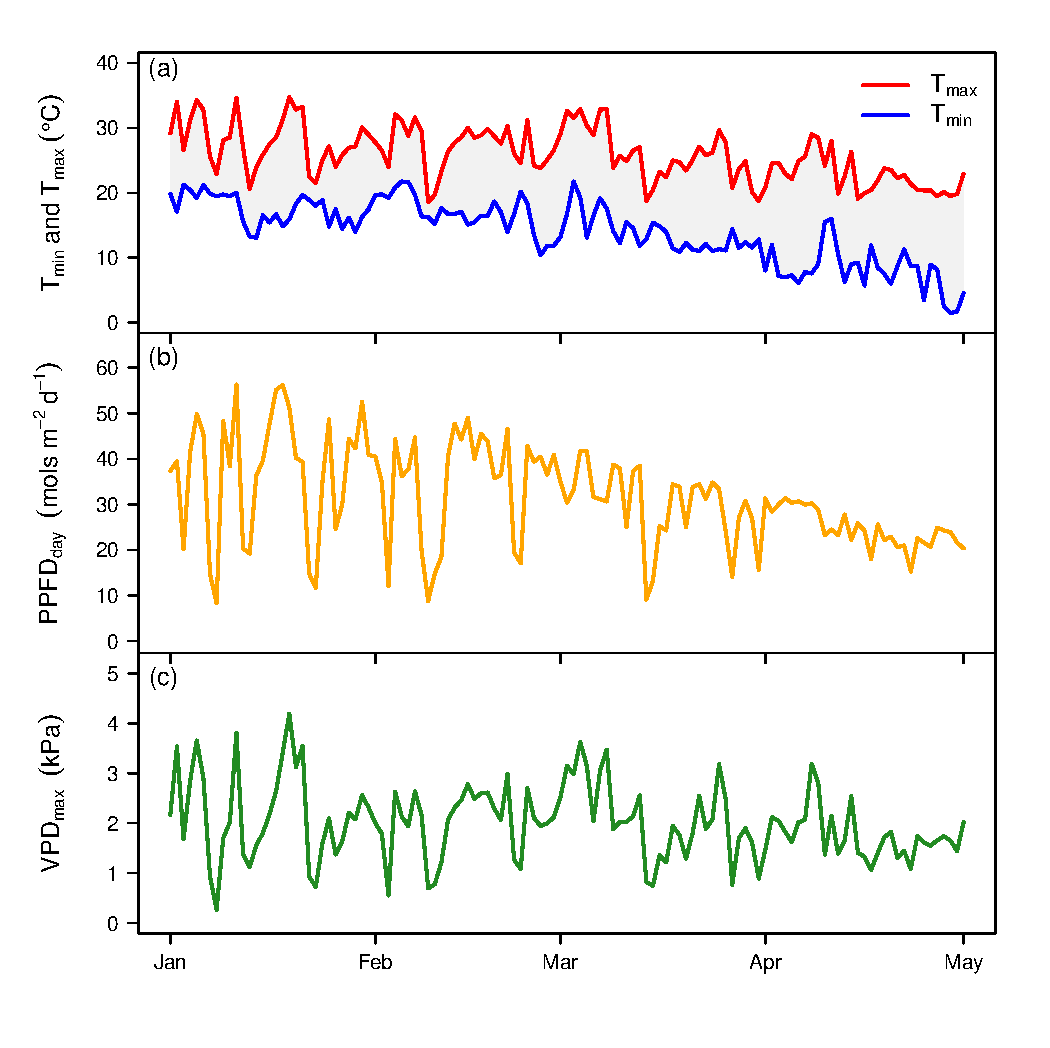
\includegraphics[width=0.99\textwidth]{airvars.pdf}
    \caption{Daily maximum and minimum temperature (a), cumulative daily PPFD (b), and daily maximum vapour pressure deficit (c) across the experiment duration in 2013.}
    \label{fig:figure1}
\end{figure}

%allometry figure
\begin{figure}[h!]
    \centering
    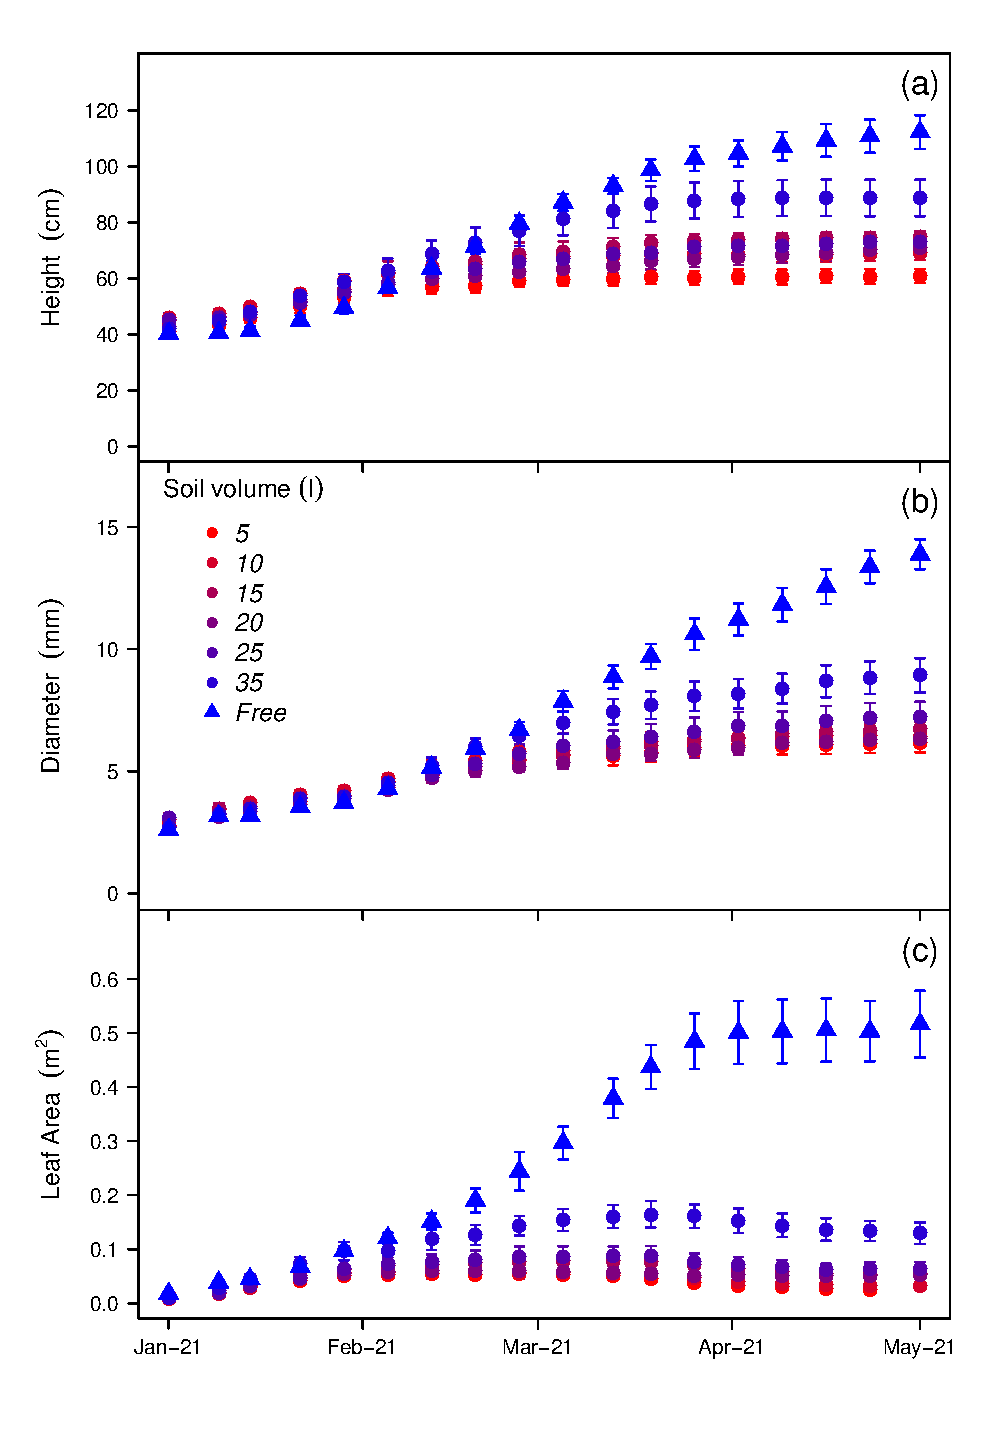
\includegraphics[width=0.99\textwidth]{allometry.pdf}
    \caption{Soil volume treatment means~$\pm$~SE~(n=7) of height growth (a), diameter growth (b), and interpolated seedling leaf area (c) measured weekly of \textit{Eucalyptus tereticornis} seedlings across the experiment duration in 2013.}
    \label{fig:figure2}
\end{figure}

%asat figure
\begin{figure}[h!]
    \centering
    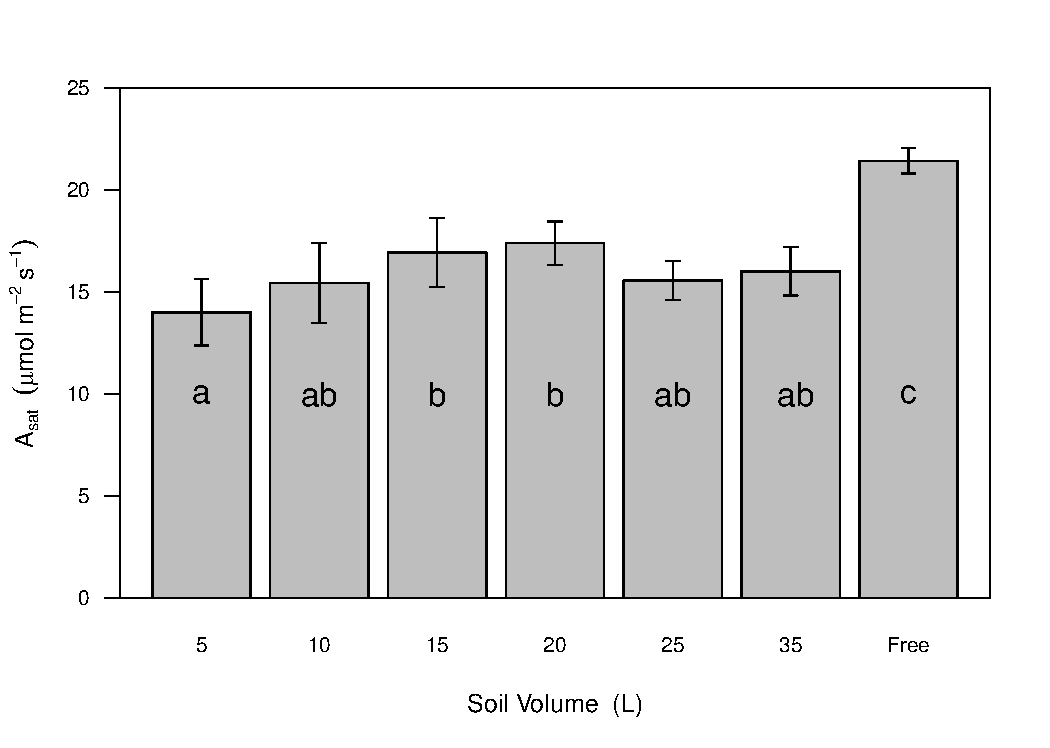
\includegraphics[width=0.99\textwidth]{Asat.pdf}
    \caption{Soil volume treatment means~$\pm$~SE~(n=7), across all measurement dates (n=6), of light saturated rates of photosynthesis at 25$\degree$C. Different letters represent significant differences between treatments.}
    \label{fig:figure3}
\end{figure}

%partitioning figure
\begin{figure}[h!]
    \centering
    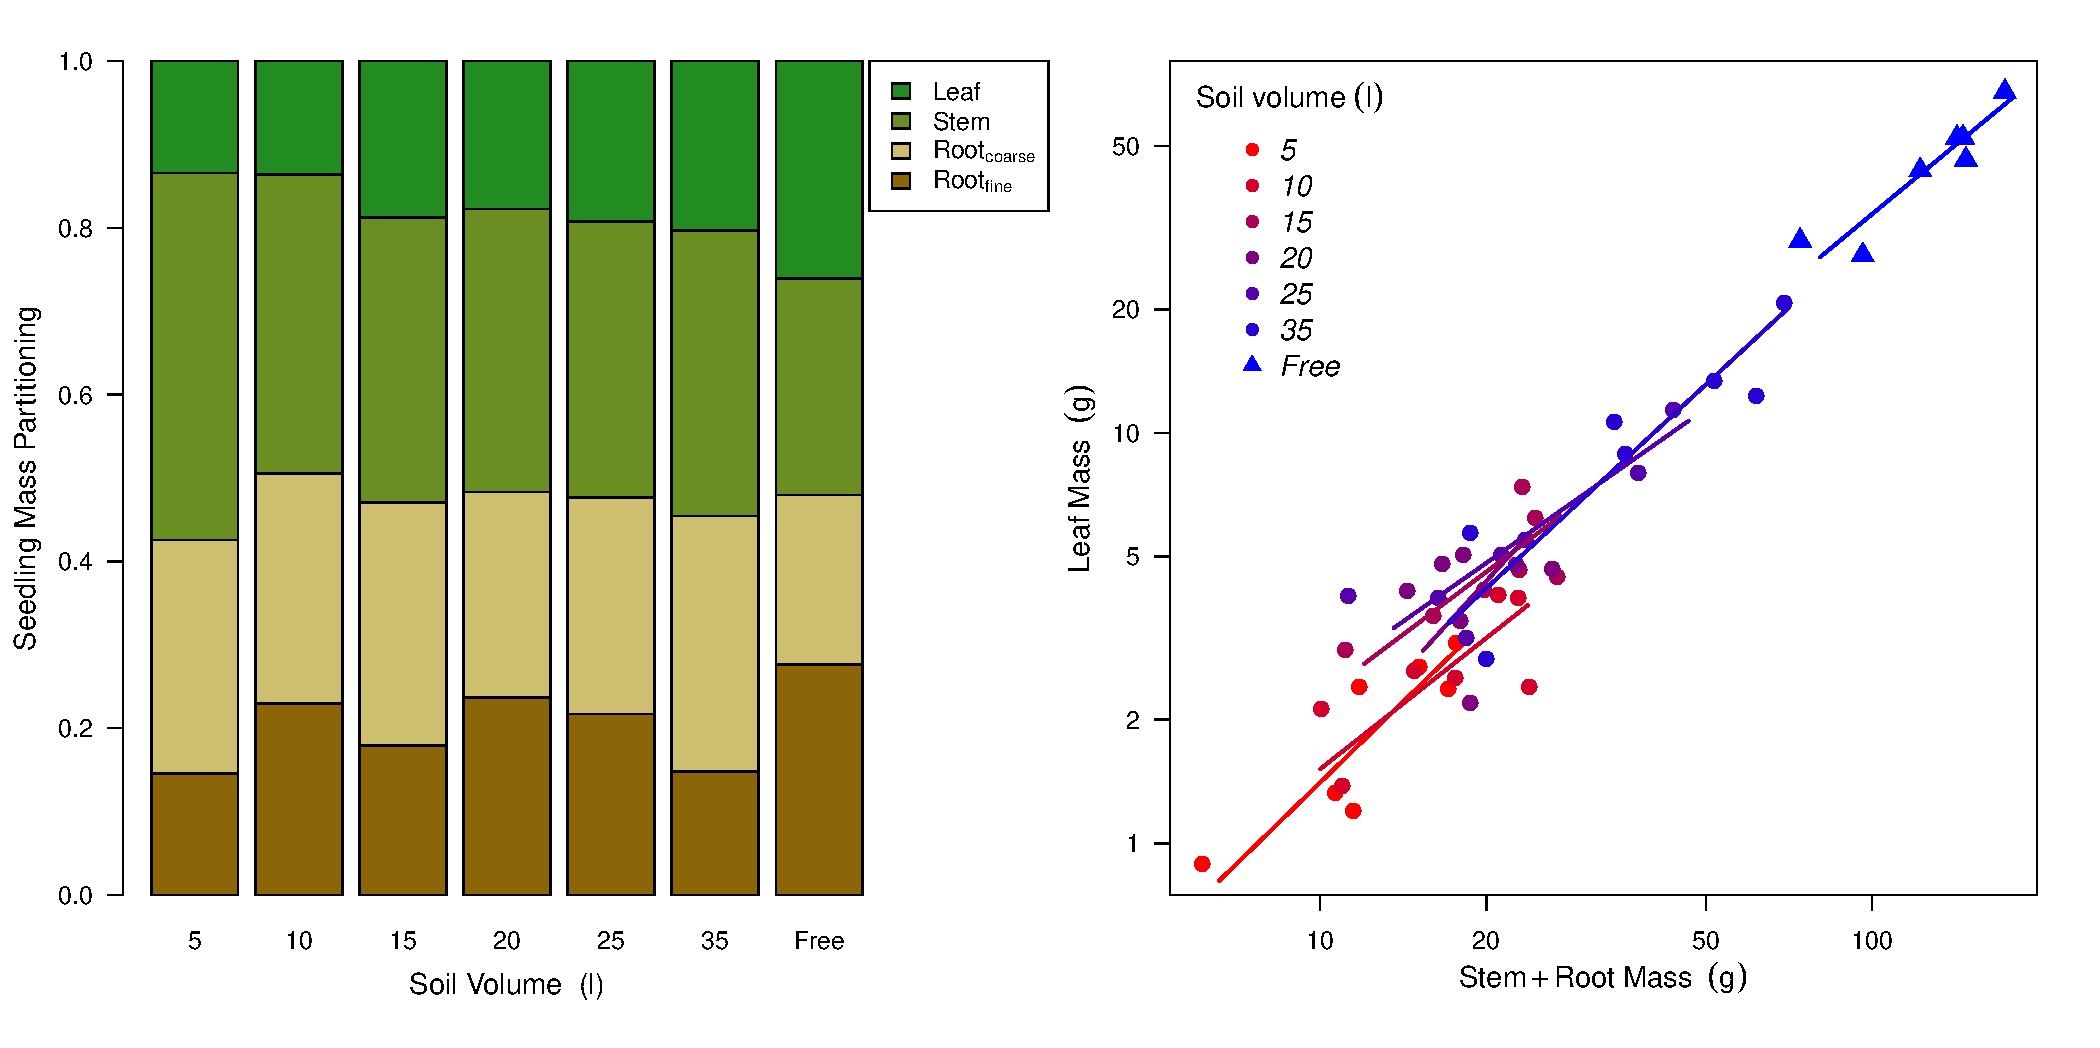
\includegraphics[width=0.99\textwidth]{massfractions.pdf}
    \caption{Soil volume treatment means (n=7) of mass partitioning to leaves, stems, and roots (a) and bi-variate relationships between mass allocation to leaves and stems + roots (b). Lines represent standardized major axis fitting of the log transformed allometric relationships of leaf mass fraction by treatment.}
    \label{fig:figure4}
\end{figure}

%photochem figure
\begin{figure}[h!]
    \centering
    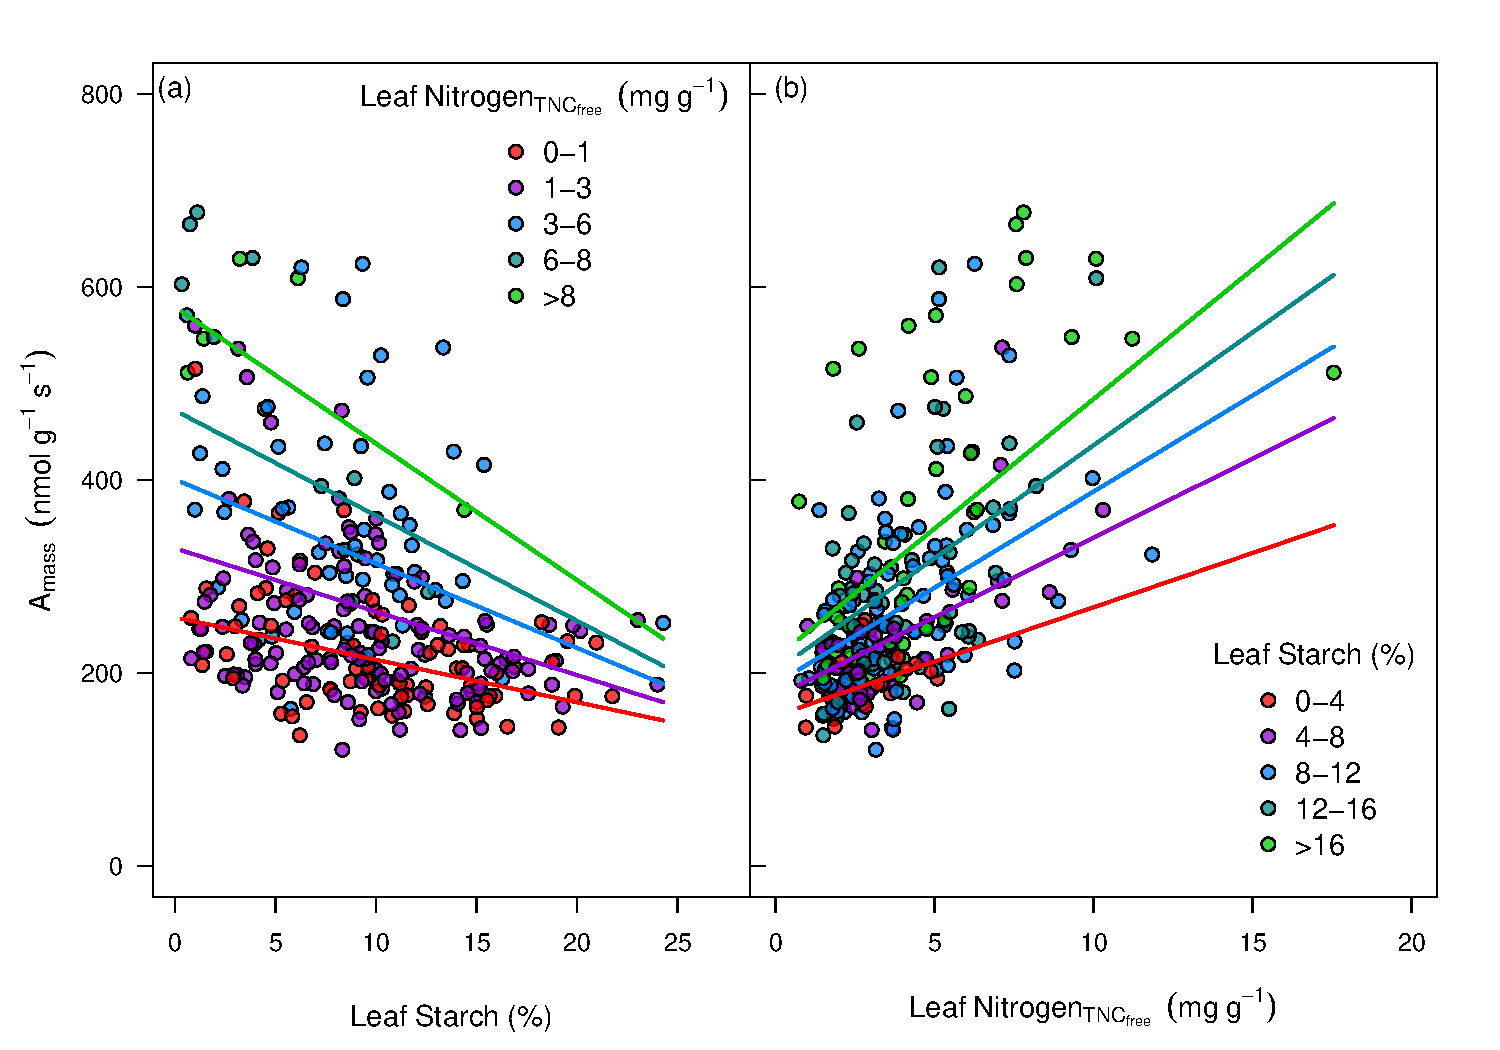
\includegraphics[width=0.99\textwidth]{A_leafchem.pdf}
    \caption{Photosynthetic capacity, on a leaf mass basis, as a function of accumulation of leaf starch (a) and leaf nitrogen content without TNC (b).  Colors represent bins levels (n=5) of both leaf starch and nitrogen grouped from low to high .  Lines represents predictions, for each bin level, from the linear mixed effects model equation of \textit{A}\textsubscript{max} as a function of starch and nitrogen. The marginal \textit{r}\textsuperscript{2} (fixed effects only) was 0.37 and the conditional \textit{r}\textsuperscript{2} (fixed and random effects) was 0.48 for the complete model.}
    \label{fig:figure5}
\end{figure}

%model base figure
\begin{figure}[h!]
    \centering
    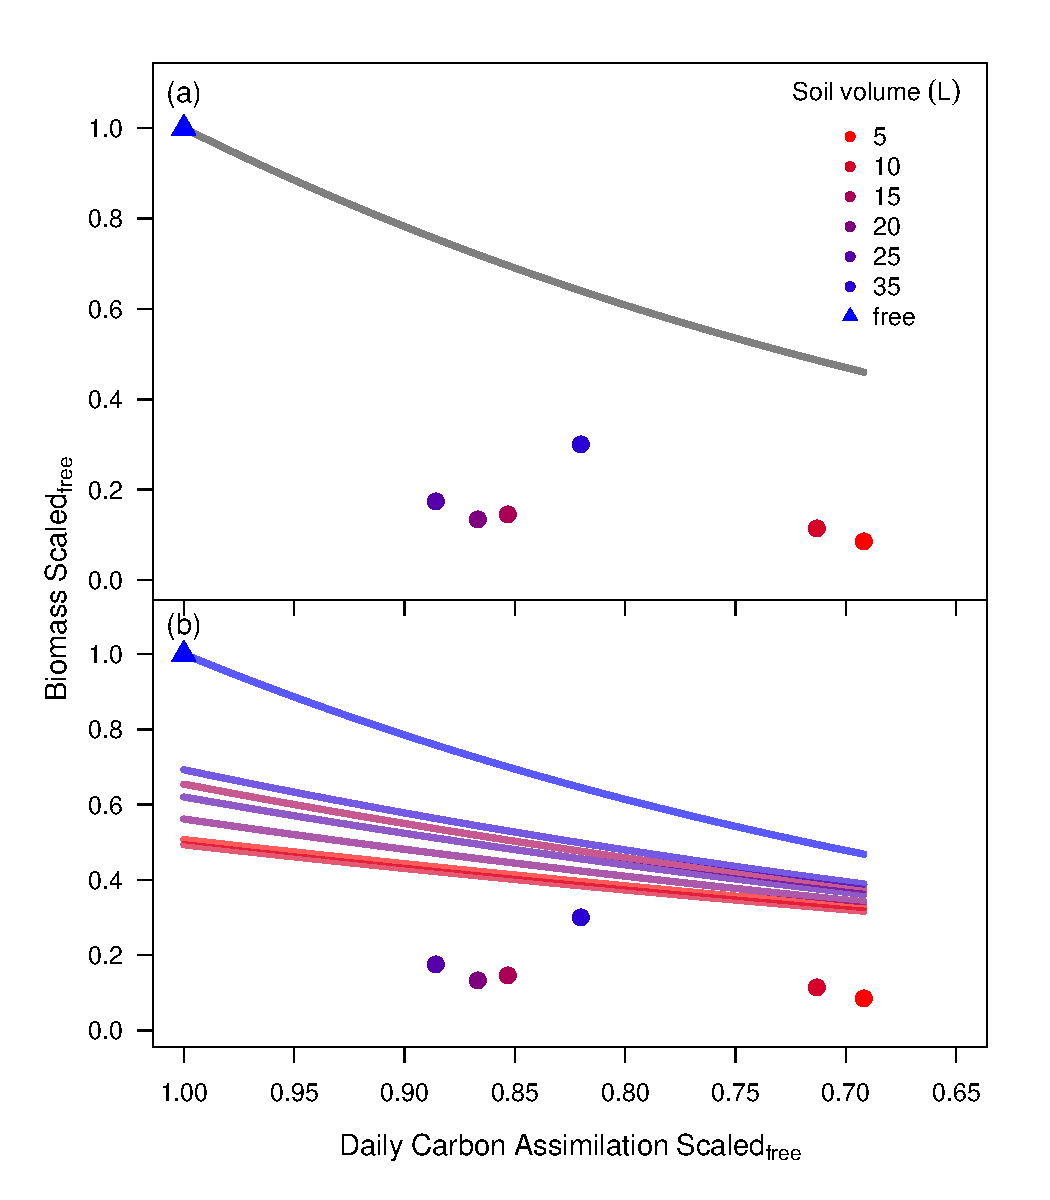
\includegraphics[width=0.99\textwidth]{gC_day.pdf}
    \caption{Modeled and harvested seedling biomass (g) versus the measure range of daily assimilated carbon gain (g~m\textsuperscript{2}) across all treatments (a) and then with treatment specific plant component mass partitioning included (b).  Values of biomass and carbon gain are scaled to the free seedling with unlimited soil volume.}
    \label{fig:figure6}
\end{figure}

%--------------------------------------------------------------------------------------------%
\clearpage
\section{Supporting Information Figures}
% Supporting information. Make sure Figures continue with Fig S1 etc.

\renewcommand\thefigure{S\arabic{figure}}    
\setcounter{figure}{0}   


\begin{figure}[h!]
    \centering
    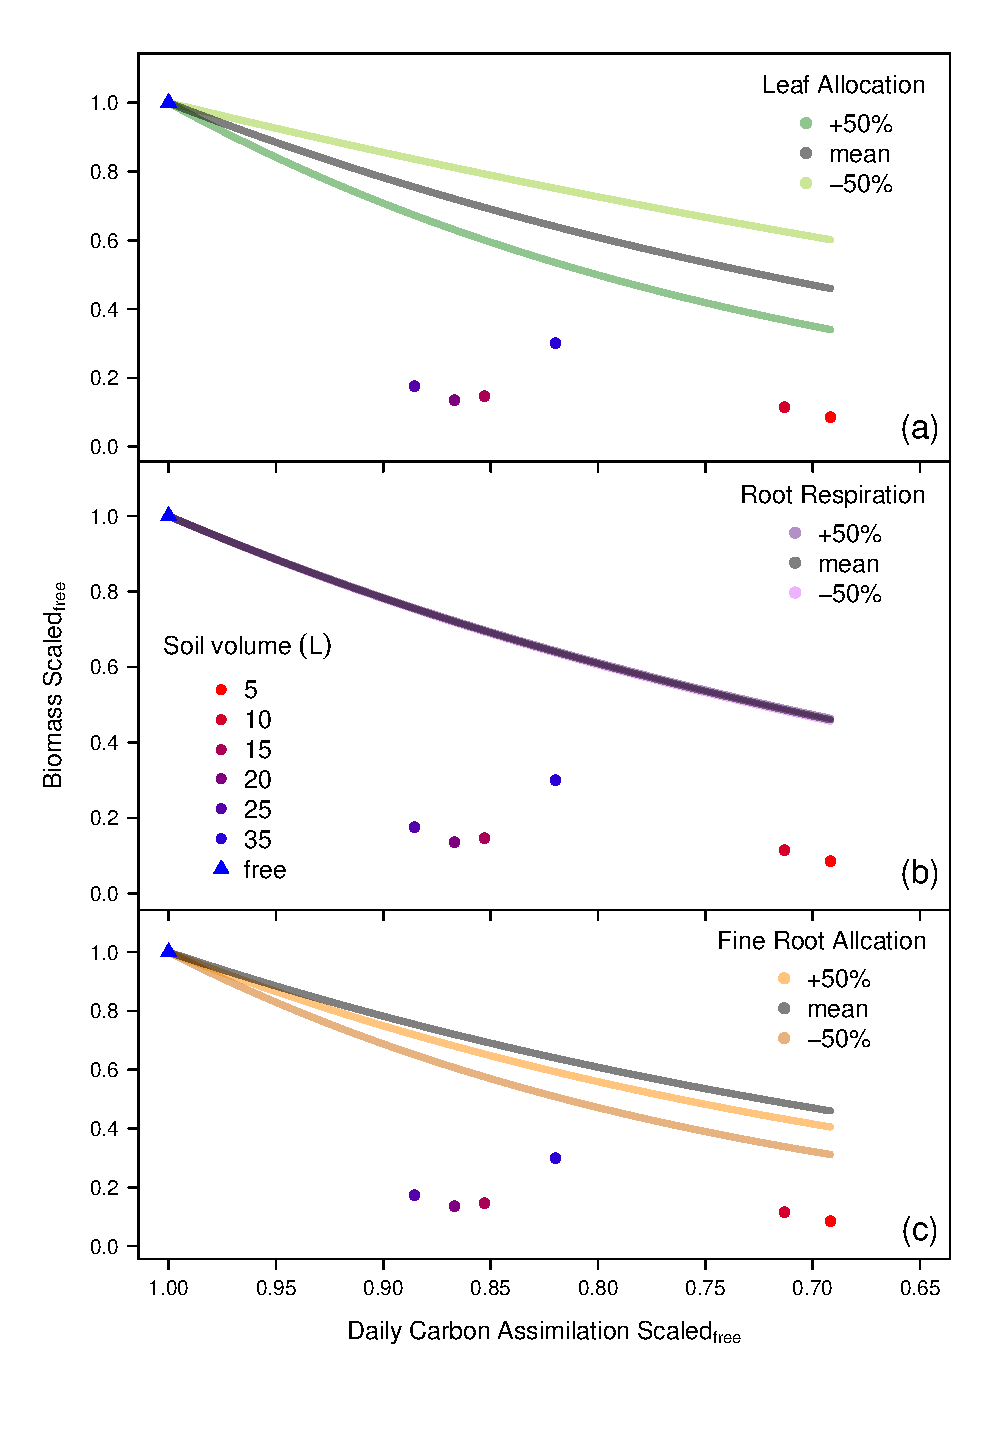
\includegraphics[width=0.99\textwidth]{gc_Day_scenario.pdf}
    \caption{Modeled and harvested seedling biomass (g) versus daily assimilated carbon gain (g~m\textsuperscript{2}) including sensitivity testing for unmeasured carbon allocation scenarios.  Model parameters of leaf allocation (a), root respiration (b), and fine root allocation (c) were increased or decreased by 50$\%$.}
    \label{fig:figureSI1}
\end{figure}


\begin{table}[h!]
  \caption{Seedling Growth Model Default Parameters} 
  \centering 
  \begin{tabular}{l l l l} 
  \hline
  Variable & Default Value & Units & Source  \\ [0.5ex] 
  \hline
  Leaf area\textsubscript{i} & 0.035 & m\textsuperscript{2} & this study \\ 
  Leaf mass\textsubscript{i} & 3.45 & g & this study \\ 
  Stem mass\textsubscript{i} & 1.51 & g & this study \\ 
  Root mass\textsubscript{i} & 0.99 & g & this study \\ 
  \textepsilon\textsubscript{c} & .65 & g~C g~mass\textsuperscript{-1} & \citet{makela1997carbon} \\ 
  R\textsubscript{coarse root} & 0.00124 & g~C g~root\textsuperscript{-1} & \citet{marsden2008relating} \\ 
  R\textsubscript{fine root} & 0.010368 & g~C g~root\textsuperscript{-1} & \citet{ryan2010factors} \\ 
  R\textsubscript{stem} & 0.00187 & g~C g~stem\textsuperscript{-1} & Drake 2014 (unpublished) \\ 
  C\textsubscript{day} & 4.7-6.8 & g~C m\textsuperscript{-2} & this study \\ 
  M & 0.80-0.87 &  & this study \\ 
  $\Lambda$ & 1/365 & yr\textsuperscript{-1} & theoretical\\
  \hline 
  \end{tabular}
  \label{table:Table3} 
\end{table}

%--------------------------------------------------------------------------------------------%
\end{document}



